\section{MODEL DESCRIPTION}
\label{sec:problemFormulation}
\noindent\uline{Platonic solids}:
The platonic solids are also called regular polyhedra have the convex polyhedra properties. 
There are exactly five regular polyhedra namely cube, tetrahedron, octahedron, dodecahedron and icosahedron (Figure \ref{fig:platonicSolids}). 
Some of the equivalent statements are used to describe the platonic solids, including all the vertices lie on a sphere, all the dihedral angle are equal, and all solid angles are equivalent. 
The tetrahedron is folded by 4-sided pyramid, the octahedron has the double-pyramid with $8$ faces and 20-sided pyramid for the icosahedron. The cube is constructed by $6$ square faces while the dodecahedron is composed of 12-sided of regular pentagons.\\

\begin{figure}[h]
\centering
	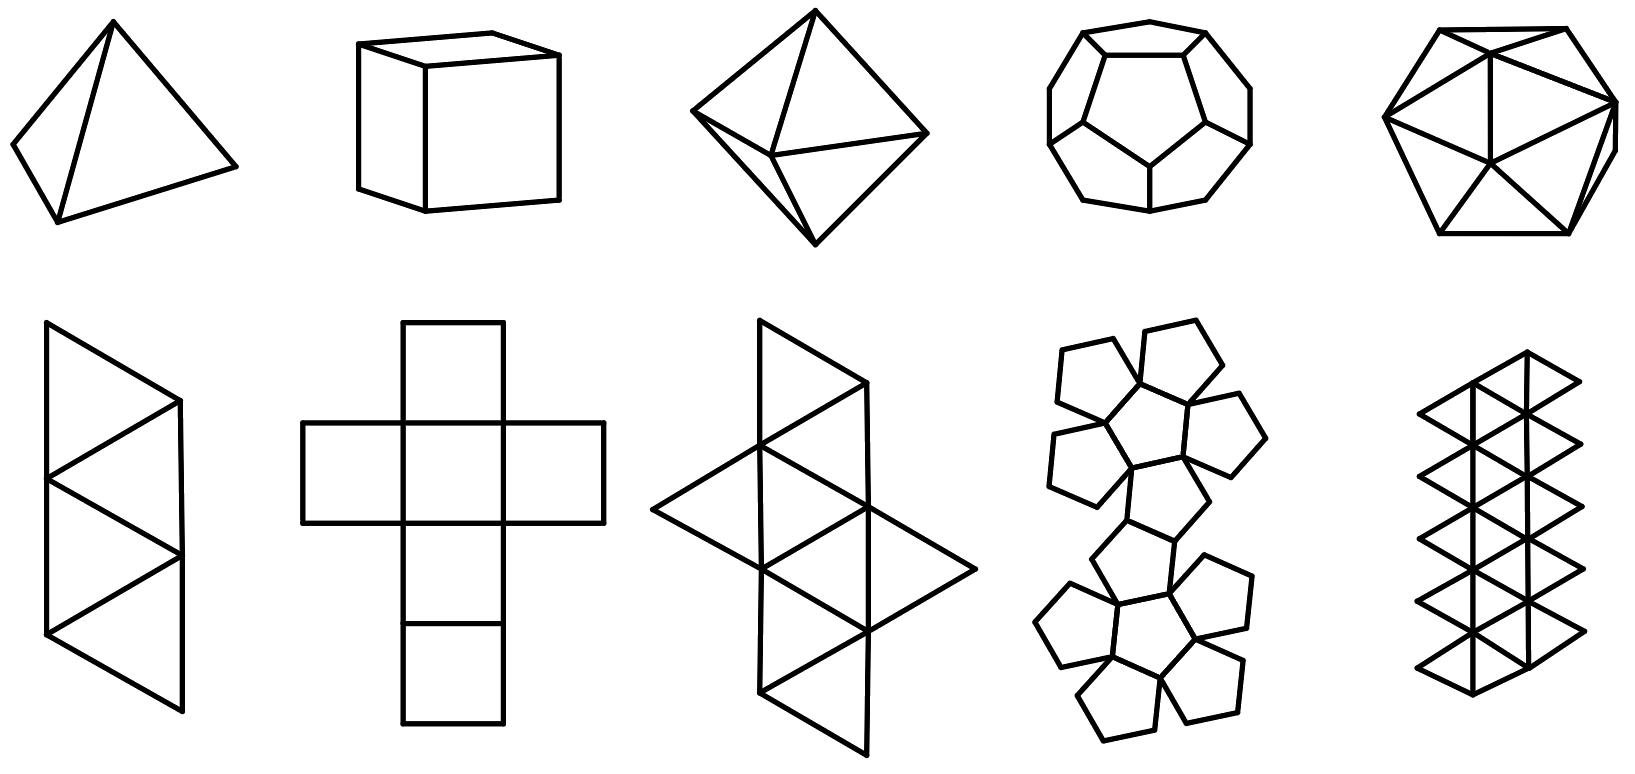
\includegraphics[width=1\textwidth]{image/5Platonic1.png}
	\caption{The platonic solids. From left to right with models and unfolding models: the tetrahedron, the cube, the octahedron, the dodecahedron, and the icosahedron}
	\label{fig:platonicSolids}
\end{figure}
%
% 
%
%
%
\noindent \uline{Geometrical parameters}: 
The number of faces, edges, and vertices of each type of platonic solids is described in the Table \ref{tab:tb1}. 
In mathematics, the Euler's formula shows the relationship between total number of vertices ($V$), edges ($E$), and faces ($F$) by the Eq. \ref{platSolProp:eq1}
%
\begin{equation} 
\label{platSolProp:eq1}
\begin{split}
V-E+F=2
\end{split}
\end{equation}
% 
The icosahedron has the largest number of faces with $20$ while the tetrahedron has only $4$ faces. 
If each face of platonic solids has $i$ sides and $k$ edges of the polyhedron meet at each vertex.
The conditions are $i,k$ greater than $3$ ($i,k\geq3$) because every face have at least three edges and at least three edges of faces meet at each vertex.
The faces are equilateral triangle if $i=3$ and changing the values of $k$ will yield the other three types of polyhedron, including the tetrahedron ($k=3$), the octahedron ($k=4$),and the icosahedron ($k=5$). When $i=4$, the faces are square and the cube has $k=3$ edges which meet at each vertex. The last case with $i=4$ of regular pentagons and only $k=3$ will generate the dodecahedron. \\

% %Check p.61 Euler's gem book
%
\begin{table}[H]
\centering
\caption{Properties of polyhedron}
\label{tab:tb1}
\begin{tabular}{|l|c|c|c|c|c|}
\hline
             & Faces & Edges & Vertices & Edges on each face & Edges meeting at each vertex \\ \hline
Tetrahedron  & 4     & 6     & 4        & 3                  & 3                            \\ \hline
Cube         & 6     & 12    & 8        & 4                  & 3                            \\ \hline
Octahedron   & 8     & 12    & 6        & 3                  & 4                            \\ \hline
Dodecahedron & 12    & 30    & 20       & 5                  & 3                            \\ \hline
Icosahedron  & 20    & 30    & 12       & 3                  & 5                            \\ \hline
\end{tabular}
\end{table}
% generate the table from https://www.tablesgenerator.com/#
%
% %Check p.61 Euler's gem book

\noindent The path planning for platonic solids focuses on the rolling of the models through edge contact. Each edge is shared by two faces and each face may has $e$ edges. Assume that $\Delta $ is the quantity faces which contact at an edge or $E=\frac{1}{2}\Delta $. However, each vertex will be shared by $f$ faces. Then, $V=\frac{\Delta}{f}$. After substituting these two quantities into the Eq. \ref{platSolProp:eq1}, the result is:
%
%
\begin{equation*} 
\label{platSolProp:eq1}
\begin{split}
V-E+F &= 2\\
\frac{\Delta}{f} - \frac{1}{2}\Delta + F &= 2\\
F &= \frac{4f}{2e-fe+2f}\\
\end{split}
\end{equation*}
%

\noindent Rotation angle is the important condition in the path planning through rolling contact. 
In the context of regular convex polyhedra, a rotation angle is supplementary with a dihedral angle which is the angle between two faces inside the polyhedra.
The Table \ref{tab:tb2} shows the radii of each solid with the inradius ($r_i$), the midradius ($\rho$), the circumradius ($R$) and the dihedral angles ($\beta$).\\

\begin{table}[h]
\centering
\caption{Geometrical parameters of platonic solids}
\label{tab:tb2}
\begin{tabular}{|l|c|c|c|c|}
\hline
             & $r_d$	                             & $\rho$                    & R	     					      & dihedral angles ($\beta$)	\\ \hline
Tetrahedron  & $\frac{1}{12}\sqrt{6}$    			 & $\frac{1}{4}\sqrt{2}$     & $\frac{1}{4}\sqrt{6}$              & $\cos^{-1}(\frac{1}{3})$                       \\ \hline
Cube         & $\frac{1}{2}$                         & $\frac{1}{2}\sqrt{2}$     & $\frac{1}{2}\sqrt{3}$              & $\frac{1}{2}\pi$                \\ \hline
Octahedron   & $\frac{1}{6}\sqrt{6}$    			 & $\frac{1}{2}$    	     & $\frac{1}{2}\sqrt{2}$      		  & $\cos^{-1}(-\frac{1}{3})$               \\ \hline
Dodecahedron & $\frac{1}{20}\sqrt{250+110\sqrt{5}}$  & $\frac{1}{4}(3+\sqrt{5})$ & $\frac{1}{4}(\sqrt{15}+\sqrt{3})$  & $\cos^{-1}(-\frac{1}{5}\sqrt{5})$              \\ \hline
Icosahedron  & $\frac{1}{12}(3\sqrt{3}+\sqrt{15})$   & $\frac{1}{4}(1+\sqrt{5})$  & $\frac{1}{4}\sqrt{10+2\sqrt{5}}$  & $\cos^{-1}(-\frac{1}{3}\sqrt{5})$               \\ \hline
\end{tabular}
\end{table}

\clearpage
\newpage
%\vspace{1in}
%\begin{table}%[h!]
%	\centering
%	\caption{Optimized Parameter Values}
%	\begin{tabular}{llllp{7em}p{7em}l}
%		\toprule
%		Type of Controller & Parameter    & Xmax & Xmin & \raggedright Iter. reqd. for convergence & Optimized value & $W_\mathrm{min}$ \\ \midrule
%			PSO-SOSMC        & $c_1$        & 5    & 0.1  & 37                                       & 4.75            & 68.43 \\
%			                 & $c_2$        & 5    & 0.1  & 10                                       & 4.273           & 20.45 \\
%			                 & $\lambda_1 $ & 5    & 0.1  & 37                                       & 2.75            & 68.43\\
%			                 & $\lambda_2 $ & 5    & 0.1  & 10                                       & 3.59            & 20.45\\
%			                 & $W_1 $       & 1    & 0.05 & 37                                       & 0.43            & 68.45\\
%			                 & $W_2 $       & 1    & 0.05 & 10                                       & 0.218           & 20.43\\ \cmidrule(lr){2-7}
%			PSO-BELBIC       & $W_1$        & 5    & 0.1  & 36                                       & 4.5             & 27.34 \\
%			                 & $W_2$        & 5    & 0.1  & 14                                       & 4.5             & 61.63 \\
%			                 & $G_1$        & 5    & 0.1  & 36                                       & 1.4             & 27.34 \\
%			                 & $G_2$        & 5    & 0.1  & 14                                       & 1.4             & 61.63\\ \bottomrule
%		\end{tabular}
%\end{table}